\documentclass[12pt, a4paper]{article}

\usepackage[utf8]{inputenc}
\usepackage[T2A]{fontenc}
\usepackage[russian]{babel}
\usepackage{geometry}
\geometry{a4paper, top=20mm, bottom=20mm, left=25mm, right=15mm}
\usepackage{graphicx}
\usepackage{tabularx}
\usepackage{booktabs}
\usepackage{hyperref}

\begin{document}

% Титульный блок
\noindent
\textbf{ALU register}\\
Александр Куртеев, ФРКТ МФТИ, kurteev.am@phystech.edu\\
4 вариант \\

\vspace{1em}

\tableofcontents

\vspace{2em}

\section{Функциональное описание}
Разработанный модуль АЛУ выполняет арифметические и логические операции над двумя операндами (\texttt{first\_i} и \texttt{second\_i}) в зависимости от заданного входного кода (\texttt{opcode\_i}). 

Устройство является синхронным, с конвейерной задержкой в один такт. Комбинационная логика вычисляет результат асинхронно, но выдача результата на выход \texttt{result\_o} происходит строго по положительному фронту тактового сигнала \texttt{clk\_i}. 

Модуль оснащен входом разрешения работы \texttt{valid\_i}. АЛУ обновляет выходной регистр данных и устанавливает флаг готовности \texttt{valid\_o} в единицу только в том случае, если в момент прихода тактового импульса сигнал \texttt{valid\_i} был активен. В таблице \ref{tab:opcode} представлено соответствие кодов операций и выполняемых действий.

\begin{table}[h]
\centering
\label{tab:opcode}
\vspace{0.5em}
\begin{tabular}{|c|l|}
\hline
\textbf{opcode\_i} & \textbf{Операция над \texttt{first\_i} и \texttt{second\_i}} \\ \hline
\texttt{2'b00} & Сложение (без знака) \\ \hline
\texttt{2'b01} & Побитовое И-НЕ (NAND) \\ \hline
\texttt{2'b10} & Арифметический (знаковый) сдвиг \texttt{second\_i} влево на \texttt{first\_i} \\ \hline
\texttt{2'b11} & second\_i != first\_i \\ \hline
\end{tabular}
\caption{Коды операций разработанного АЛУ}
\end{table}

\newpage

\section{Структурная схема}

\begin{figure}[h]
    \centering
    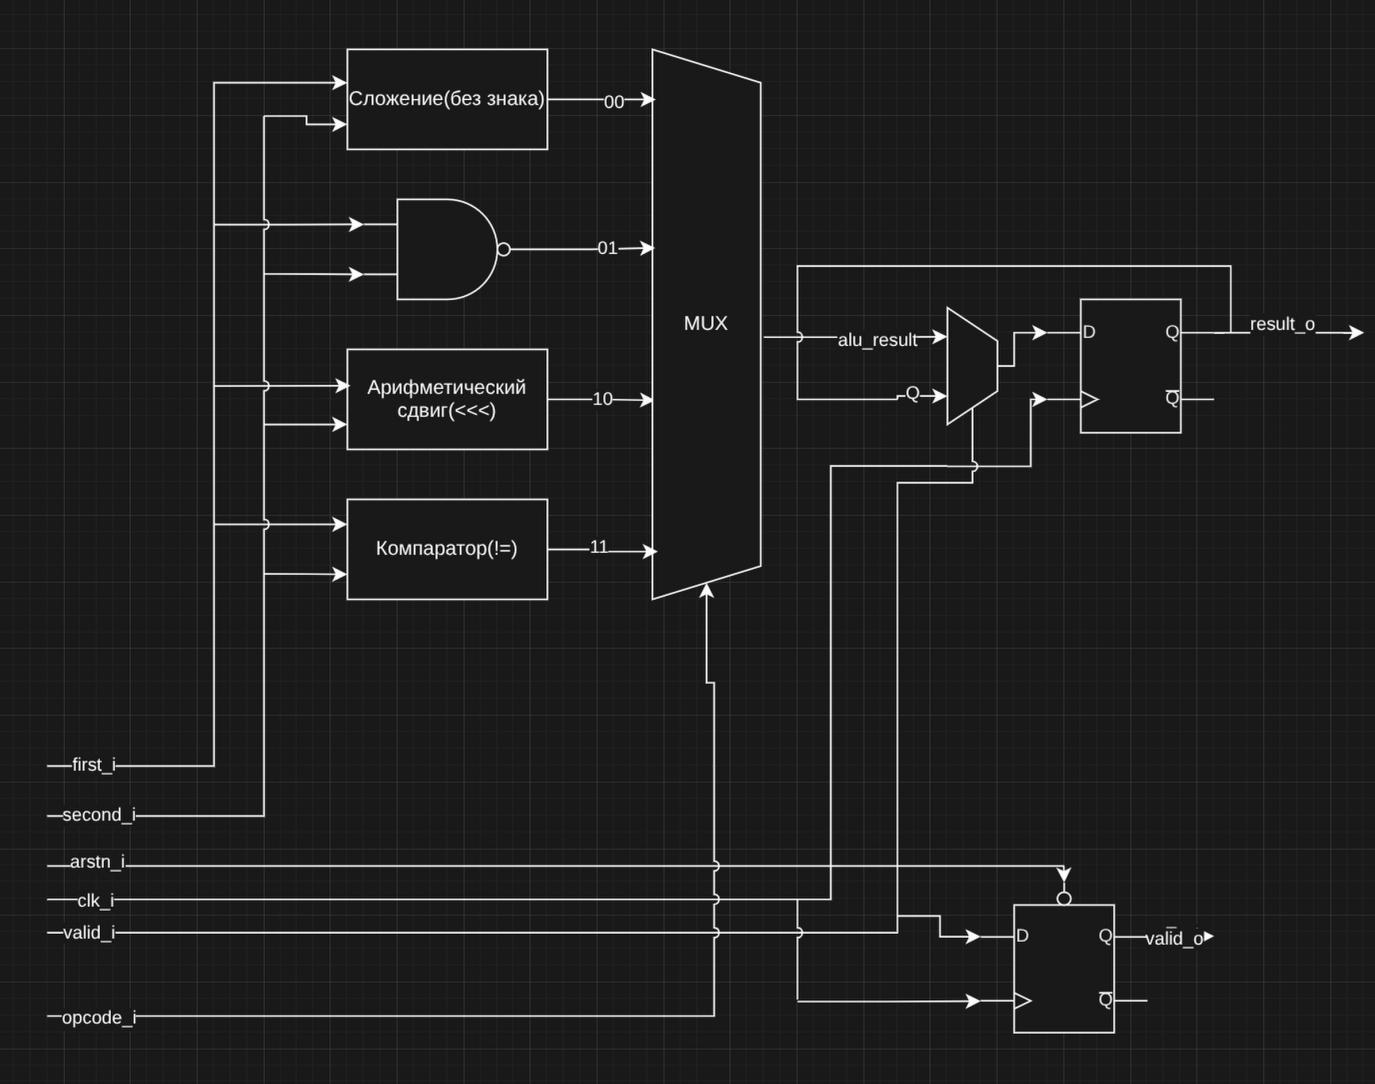
\includegraphics[width=1\textwidth]{alu_diagram.png}
    \caption{Структурная схема АЛУ}
    \label{fig:diagram}
\end{figure}

\section{Параметры}
\begin{table}[h]
\centering
\vspace{0.5em}
\begin{tabular}{|l|c|l|}
\hline
\textbf{Название} & \textbf{Значение} & \textbf{Описание} \\ \hline
\texttt{WIDTH} & По умолчанию 8 & Разрядность входных операндов и результата \\ \hline
\end{tabular}
\caption{Описание параметров}
\end{table}

\newpage

\section{Порты}
\begin{table}[h]
\centering
\vspace{0.5em}
\begin{tabular}{|l|c|l|}
\hline
\textbf{Название} & \textbf{Ширина} & \textbf{Описание} \\ \hline
\texttt{clk\_i} & 1 & Тактовый сигнал \\ \hline
\texttt{arstn\_i} & 1 & Асинхронный инверсный сигнал сброса \\ \hline
\texttt{valid\_i} & 1 & Разрешение работы (валидность данных) \\ \hline
\texttt{opcode\_i} & 2 & Код выполняемой операции \\ \hline
\texttt{first\_i} & \texttt{WIDTH} & Первый операнд \\ \hline
\texttt{second\_i} & \texttt{WIDTH} & Второй операнд \\ \hline
\texttt{valid\_o} & 1 & Флаг готовности выходных данных \\ \hline
\texttt{result\_o} & \texttt{WIDTH} & Результат операции \\ \hline
\end{tabular}
\caption{Описание портов}

\end{table}

\section{Тактирование и сброс}
Тактирование схемы осуществляется по положительному фронту сигнала \texttt{clk\_i}. Запись в выходные D-триггеры производится только при условии \texttt{valid\_i == 1}.

Сброс модуля реализован как асинхронный и инверсный через порт \texttt{arstn\_i}. При переходе \texttt{arstn\_i} в логический нуль происходит немедленный сброс управляющего триггера (\texttt{valid\_o} обнуляется) независимо от тактового генератора. Регистр данных \texttt{result\_reg} при сбросе не обнуляется для оптимизации, так как логика следующего уровня конвейера ориентируется на флаг \texttt{valid\_o}.

\section{Тестирование}
Верификация модуля выполнена с использованием testbench-файла. В блоке \texttt{always} реализован генератор тактового сигнала с заданным периодом.

Процедура тестирования:
\begin{enumerate}
    \item Выполняется обнуление всех входных сигналов.
    \item Модуль удерживается в состоянии сброса (\texttt{arstn\_i = 0}), после чего сброс асинхронно снимается.
    \item Для предотвращения состояния гонки  в симуляторе, подача тестовых векторов (сигналов \texttt{first\_i}, \texttt{second\_i}, \texttt{opcode\_i} и \texttt{valid\_i}) осуществляется по спаду тактового сигнала (\texttt{negedge clk\_i}).
    \item На следующем спаде тактового сигнала команда снимается (\texttt{valid\_i = 0}).
    \item На временных диаграммах контролируется появление корректного результата на шине \texttt{result\_o} с задержкой ровно в один такт и его успешное удержание в регистре. Процедура повторяется для всех операций.
\end{enumerate}

\begin{figure}[h]
    \centering
    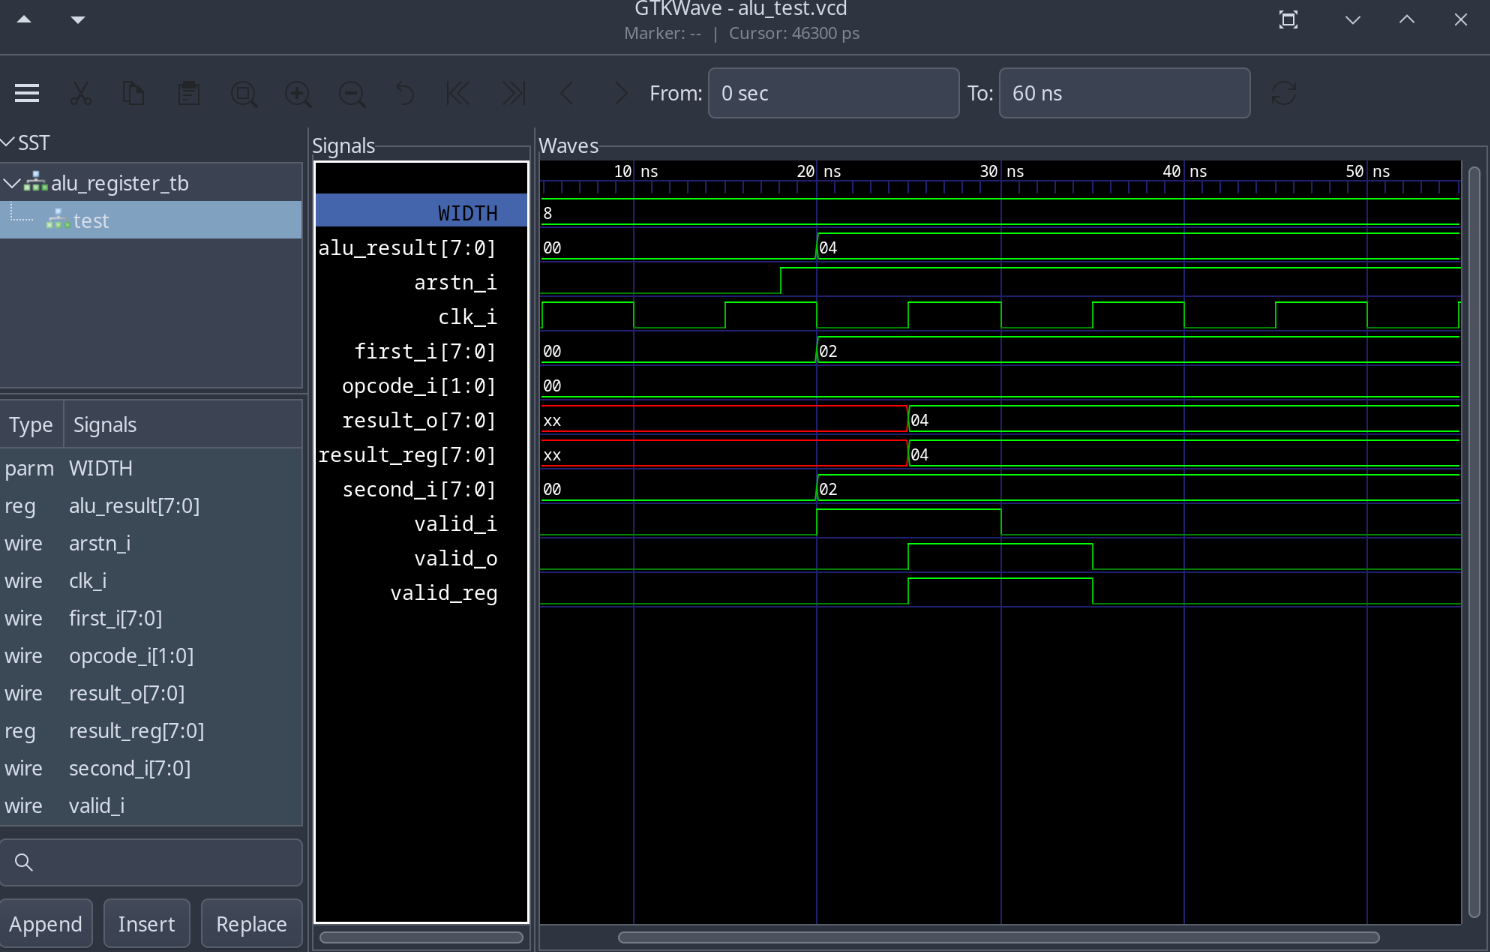
\includegraphics[width=1\textwidth]{gtk_diagram.png}
    \caption{Временная диаграмма}
    \label{fig:diagram}
\end{figure}


\end{document}